% !TEX root = ./summary.tex

\section{Einrichten von \antlr auf Eclipse}
In diesem Kapitel geht es darum \antlr herunter zu laden, um es danach in Eclipse zu integrieren. 

\subsection{Schritt 1 - \antlr herunterladen}
\label{sec:step1}
\antlr von \href{http://www.antlr.org/download}{http://www.antlr.org/download} herunterladen. Am besten nimmt man dazu die \textbf{antlr-X.X.X-complete.jar}. Wenn die Source Attachments unbedingt eingesehen werden mu"ssen, kann auch noch das .zip u"ber \href{http://www.antlr.org/download.html}{http://www.antlr.org/download.html} heruntergeladen werden.\\
\textbf{Es ist wichtig diese Dateien irgendwo abzulegen, wo sie immer wieder gefunden werden k"onnen.}

\subsection{Schritt 2 - \antlr Plugin installieren und einrichten}
\label{sec:step2}
F"ur \antlr gibt es ein Plugin, welches sich leicht auf dem Eclipse Marketplace finden l"asst. Man muss dazu einfach \antlr in dessen Suche eingeben und dann auf installieren klicken.

\begin{figure}[H]
	\centering
	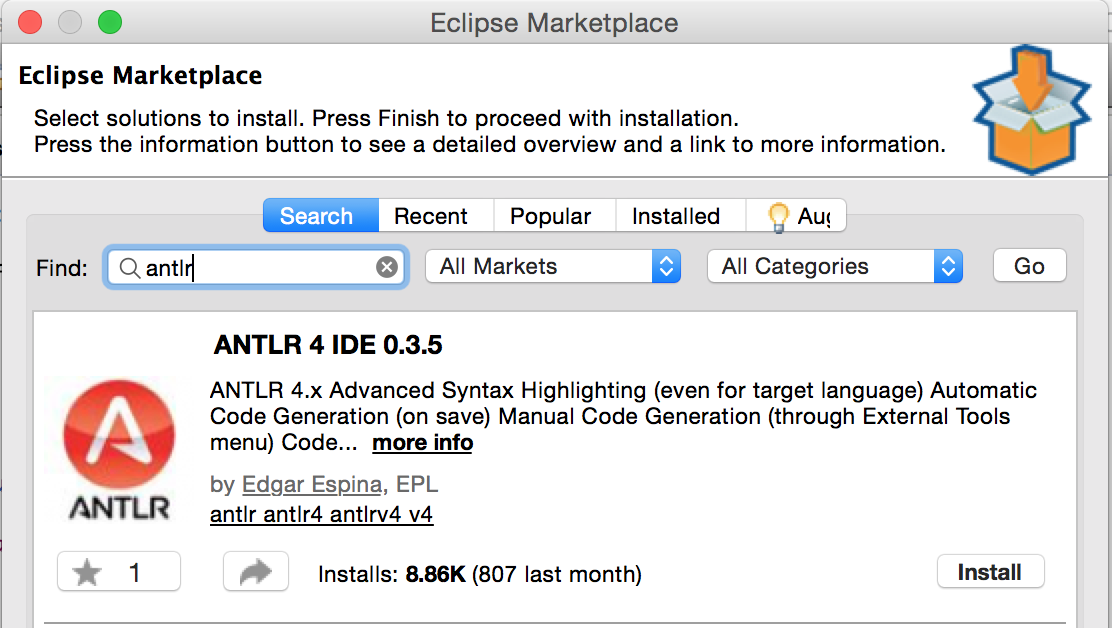
\includegraphics[width=0.65\textwidth]{antlr_plugin}
	\caption{\antlr Plugin im Eclipse Marketplace}
\end{figure}

Als n"achstes muss das Plugin noch eingerichtet werden. 

\begin{figure}[H]
	\centering
	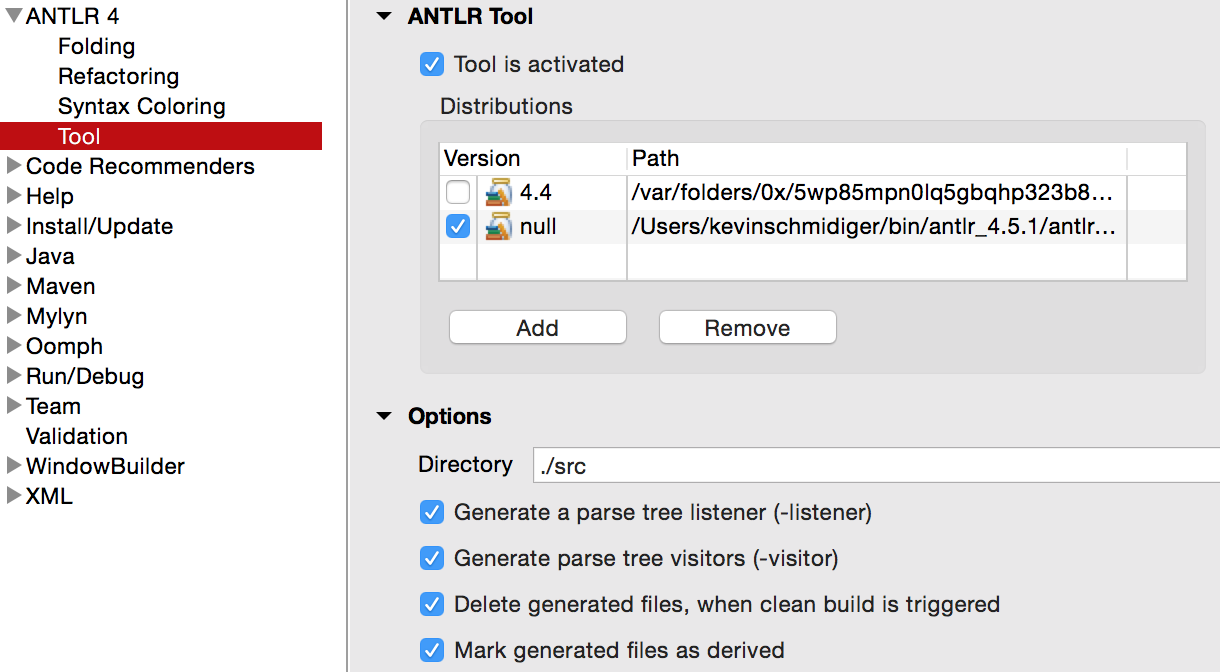
\includegraphics[width=0.65\textwidth]{antlr_config}
	\caption{\antlr Konfigurationsmenu}
\end{figure}

Es ist zu beachten, dass das Directory ge"andert wird zu ./src. Das ist der Ausgabeort von dem von \antlr generiertem Code. Auch w"urde ich die default Version wechseln zu der, die in Kapitel~\ref{sec:step1} heruntergeladen wurde. 

\subsection{Schritt 3 - Projekt aufsetzen}
Ein neues Projekt aufsetzten ist nicht schwirig. Man muss nur ein normales Java Projekt erstellen und eine gewisse Ordnerstruktur einhalten und auch die entsprechenden Libraries einbinden. 

\begin{figure}[H]
	\centering
	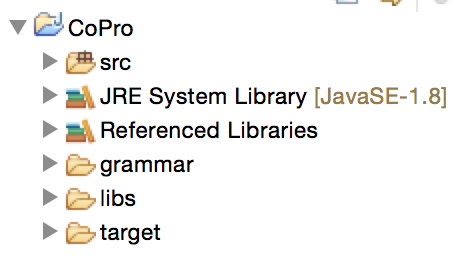
\includegraphics[width=0.65\textwidth]{structure}
	\caption{\antlr Ordnerstruktur}
\end{figure}

Die Ordnerstruktur ist wie gehabt, es kommen einfach die Ordner target und grammar hinzu (sowie libs oder lib was auch nicht un"ublich ist in Java Projekten). Im weiteren werden kurz auf die Ordner und deren Aufgaben eingegangen.

\subsubsection{Ordner grammar}
Logischerweise ist in dem Ordner grammar die Grammatik definiert, welche eine .g4 Datei ist. 

\begin{figure}[H]
	\centering
	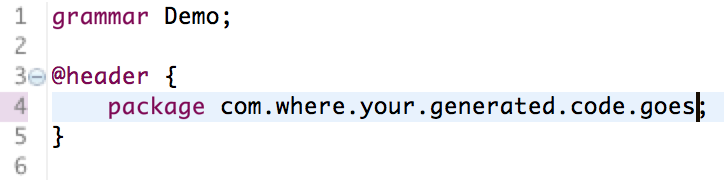
\includegraphics[width=0.65\textwidth]{grammar_file}
	\caption{\antlr Grammatikdatei}
\end{figure}

Die erste Zeile definiert, dass es eine Grammatik ist. Das @header gibt in diesem Fall an, wohin den von \antlr generierten Code hin soll. Da schon bei der Konfiguration des Plugins im Kapitel~\ref{sec:step2} im Directory ./src angegeben wurde, generiert es den code in diesen Ordner und dann in das entsprechende Package. Nach dem Header folgt dann die eigentliche Grammatik.

\subsubsection{Ordner target}
In diesem Ordner hat es eine .demo Datei, welche den Code, welcher in der Grammatik definiert wurde, kompiliert werden sollte. Diese Datei kann man auch brauchen, um den Abstrakten Syntax Baum (\href{https://en.wikipedia.org/wiki/Abstract_syntax_tree}{eng. Abstract Syntax Tree AST}) darzustellen, worauf sp"ater in Kapitel~\ref{sec:visualizeAST} genauer eingegangen wird. \\

So, nun ist man soweit, um voll loslegen zu k"onnen. Als n"achstes stehen die Visualisierung vom dem Syntax Baum an, sowie man denn nun einen Parser f"ur die Grammatik schreibt. 